%\documentclass[letterpaper, twocolumn]{article}
\documentclass[letterpaper]{article}

% Change the margins to 1 inch all around.
\usepackage[margin=1in]{geometry}

% font handling
%\usepackage{fontspec}

% for setting the linespace (\setstretch)
\usepackage{setspace}

% distance between the columns
\setlength{\columnsep}{1cm}

% for compactitem
\usepackage{paralist}

% for comments
\usepackage{verbatim}

\usepackage{booktabs}
\usepackage{longtable}
\usepackage{float}
\usepackage{graphicx}
\usepackage{hyperref}
\usepackage{listings}
\usepackage{amsmath}
\usepackage{tcolorbox}
\usepackage{amssymb}

\usepackage[
	sorting=none,
	minbibnames=8,
	maxbibnames=9,
	block=space,
	backend=biber
]{biblatex}
\bibliography{bibliography}

\usepackage{lipsum}

\begin{document}

% Blue text box for answers.
\newtcolorbox{myanswerbox}[1][]{
  colback=blue!5!white, % Background color
  colframe=blue!75!black, % Bourder color
  fonttitle=\bfseries, %  Font style of the title
  title=#1, %  Title
  arc=0mm, %  Rounded corners
  #1
}

\lstset{
    language=Python,
    basicstyle=\ttfamily\small,
    keywordstyle=\color{blue},
    backgroundcolor=\color{lightgray}
}

%=============================
{
	\parindent0pt
	\setstretch{1.4}
	\ \\ \ \\ \ \\

	\hrulefill
	\vspace{0.0cm}
	\begin{spacing}{2.1}
	{	
		\flushleft
		\fontsize{22pt}{44pt}\selectfont 
		Homework 3: Aggregte Demand, Aggregate Supply and General Equilibrium
	}\\
	\textsc{Microeconomics - ECON 401A}
	\end{spacing}

	\ \\ \ \\
	{
		\setstretch{1.2}
		\textbf{Mauricio Vargas-Estrada}\\
		\textbf{Santiago Naranjo Manosalva}\\
		Master in Quantitative Economics\\
		University of California - Los Angeles\par
	}
	\ \\

	\hrulefill

}

{
	\setstretch{1.1}
	{\bfseries
	This project, led by Mauricio Vargas and Santiago Naranjo, will focus on providing an understanding of how prediction markets operate in the realm of cryptocurrencies. Specifically, we will explore the functioning of Winner-Take-All contracts, where the object of interest is the occurrence of an event. The study of prediction markets is crucial, as they serve as a vital tool for gauging market expectations. It is theorized that they can assimilate all available information effectively through the involvement of numerous agents, thereby forming a collective projection. Throughout this text, we will delve into the interactions among various participants in the prediction markets, explore how predictions are formulated, and use specific examples from Polymarket to examine relevant hypotheses regarding these markets such as their level of efficiency, arbitrage opportunities, and their low susceptibility to manipulation.
	The analysis undertaken in this study encompasses a qualitative examination of key research in the field of Crypto-predictive markets, complemented by a quantitative analysis of data sourced from leading prediction market platforms, with an emphasis on Polymarket. To address the core questions of the study, variables such as historical pricing, trading volumes, and contract details are scrutinized. This approach allows for a thorough investigation into the prevailing trends and behavioral patterns evident in these markets.
}\par

}
\newpage

%=============================
\section{Introduction}
\label{sec:introduction}

\lipsum[2]

\section{Predictive Markets}
\label{sec:predictive_markets}
A prediction market, as commonly defined and the focus of this work, is a market where participants can trade and exchange contracts, and the payoffs are contingent on the outcomes of future events(/citeauthor{wolfers2004prediction}). This type of market has caught the attention of the media and various technology companies in recent years due to its ability to make more accurate predictions through its pricing. According to an article from /textcite{Roose_2023}, "Prediction markets offer a better way to search for truth — rewarding those who are good at forecasting by allowing them to make money off those who are bad at it, while settling on the facts in an unbiased way".

\lipsum[2]

\subsection{Winner-Takes-All Contracts}
\label{subsec:winner_takes_all_contracts}

\lipsum[2]

\section{Crypto-Predictive Markets}
\label{sec:crypto_predictive_markets}

The Crypto-Predictive Markets are a special type of decentralized finance where blockchain infrastructure is used to define smart contracts that can later be traded without the need for an intermediary, using some type of cryptocurrency as the exchange currency \parencite{HassanAmmar2023Fttt}. All transactions are recorded within the blockchain's ledger, being accessible to anyone who has a copy of the network. Additionally, there are special web browsers that allow viewing the records, filtering the information according to the user's needs. Below, we explore some basic concepts and how such infrastructure is employed in the context of predictive markets using Winner-Takes-All (WTA) type contracts.

\subsection{Basic Concepts}
\label{subsec:basic_concepts}

To understand the operation of a Crypto-Predictive Market, it is necessary to define some concepts that will later be used to describe how this infrastructure can be adapted in the context of WTA-type predictive market.

\subsubsection{Blockchain, Cryptocurrency and Layers}
\label{subsubsec:blockchain}

Commonly transactions are recorded in a ledger, which is an accounting book that records all transactions made. In the context of blockchain, this ledger is a distributed record among all the nodes of a network, which function as a redundant storage system. The term arises from the need to separate this record into blocks, in such a way that the handling of information is more efficient. Since the ledger or accounting book must be consistent throughout each block, they are chained together by a unique key called a hash.

In some blockchain protocols, layers are defined, so that the primary layer handles general records, while secondary layers handle specific records, which can be referenced from the primary layer without the need to record them directly. In the secondary layer, special rules can be defined for the management of records, such as the definition of a smart contract.

The process of recording a block in the ledger requires that a unique key be generated to chain the blocks. This generation of keys is not automatic, but requires the computation of keys through computational power. Different blockchains implement tokens called cryptocurrencies, which are used as rewards for the nodes that perform the computation of the keys. This process is called mining, and it is the way in which the consistency of the ledger is maintained throughout the network. Because the records in the ledger can represent real transactions, there is a monetary equivalence for cryptocurrencies, due to the added value of recording the transaction.

\subsubsection{Smart Contracts}
\label{subsec:smart_contracts}

A smart contract is a program embedded in the secondary layer of the blockchain. This contract contains the rules and deadlines that will enforce the promise of an agreement between two or more parties. These contracts do not require a legal intermediary to mediate between the parties, and the defined execution conditions are validated by a network of specialized agents known as oracles \parencite{alma9919406254106531}.

\subsubsection{Oracles}
\label{subsubsec:oracles}

Smart contracts typically establish execution conditions that require information not recorded within the blockchain. The inclusion of such external information and its tracking within the blockchain is not efficient, so a solution to this problem is to use agents that follow and validate the external information. When the contract's execution condition is met, these agents inform the contract that the condition has been fulfilled, and through a voting system, a consensus is reached among information validating agents as to whether the condition was met or not. These agents are called oracles \parencite{HassanAmmar2023Fttt}.
    
Oracles can be human agents or programs external to the blockchain. To validate a contract's condition, oracles must stake a certain amount of money, usually in the form of cryptocurrencies. Those who correctly validate the information receive a reward, while those who do not lose the money staked.
    
The more oracles a smart contract has, the more robust the results will be, and the lower the probability that a malicious oracle can alter the outcome. The number of oracles needed depends on the nature of the contract. For example, the outcome of an official Champions League football match may require few oracles, with applications connected to official information sources. On the other hand, validating hypotheses or opinions may require a larger number of oracles, due to the inherent subjectivity of the information.

\subsection{Crypto-Predictive Markets}
\label{subsec:crypto_predictive_markets}

In a Crypto-Predictive Market, a smart contract is used to define the rules of a market, setting the conditions under which a market is considered resolved. Agents can participate in the market, buying and selling shares according to their beliefs. When the market is resolved, those agents who bought shares in accordance with the correct outcome receive a reward, while those who bought shares based on an incorrect outcome lose the money staked. Oracles are used to validate the outcome of this market, which, according to the terms defined in the smart contract, receive a reward or are penalized for the correct or incorrect validation of the contract's execution condition.
    
A special type of contract is the Winner-Takes-All (WTA). In the context of a smart contract, this specific type uses a binary execution condition, either fulfilled or not fulfilled. The price of the shares is set between 0 and 1, and those agents who bought shares according to the correct outcome receive a reward of 1, having a gain of $1-p$, where $p$ is the price at which they bought the share.

\subsection{Polymarket}
\label{subsec:polymarket}


\lipsum[2]

\subsubsection{Supply and Demand Mechanism}
\label{subsubsec:supply_and_demand_mechanism}

\lipsum[2]
\section{Revising the Assumptions About Predictive Markets}
\label{sec:revising_assumptions}

\subsection{Efficency and Arbitrage opportunities}
\label{subsec:efficency_and_arbitrage_opportunities}

Predictive markets, such as Polymarket, should theoretically work well and be very efficient, so arbitrage opportunities would not be expected to be persistent(\citeauthor{luckner2008arbitrage}). These are designed to be extremely efficient because they combine data from a wide range of participants, which results in the formation of prices that accurately reflect the likelihood of future events. This implies that market participants seeking to capitalize on these differences should quickly eliminate any price discrepancies that could create arbitrage opportunities.

However, it is essential to understand that no market can operate perfectly all the time. In practice, brief arbitrage opportunities may arise because information updates are delayed, market liquidity constraints are imposed, or market participants' responses to new information are delayed. Fast and agile arbitrageurs can exploit these opportunities, although rare and usually short-lived in efficient predictive markets.

Based on the data gathered by \citeauthor{kapp2023improved} in their study on the accuracy of Polymarket, arbitrage opportunities appear to increase as the time frame for the occurrence of the event extends. This is because as the agreed-upon date for the event draws nearer, more information becomes available, and the predicted probability aligns more closely with the actual likelihood, eliminating arbitrage options. Additionally, these data reveal a clear relationship between arbitrage opportunities and the volume of contracts. Markets with a low volume of transactions, lacking a considerable number of agents, tend to be less efficient, and their prices often deviate more from the actual probability of the event, thus creating clear arbitrage opportunities. From the foregoing and the data available on Polymarket, we can assert that in mature markets with high agent participation, arbitrage opportunities tend to be nonexistent.

Because user bases and skill levels vary, so do market expectations and pricing, it is possible to explain the discrepancy in prices across various predictive markets. Furthermore, the efficiency of price adjustments is influenced by platform-specific variations in liquidity. Price disparities can also be caused by the dissemination and processing of information, transaction costs, and platform usability, as these factors can influence trader participation and market efficiency. These elements may contribute to the persistence of price disparities, particularly in more closed markets.

On the other hand, the presence of a potential arbitrage opportunity between predictive markets is observed, as seen in Image 1 obtained from \citeauthor{lPolack}, where the occurrence of a discovery in the superconductor sector is questioned. Although the question and criteria are the same, there is a discrepancy in the market price between the Metaculus, Manifold, and Polymarket platforms.

\begin{figure}[H]
    \centering
    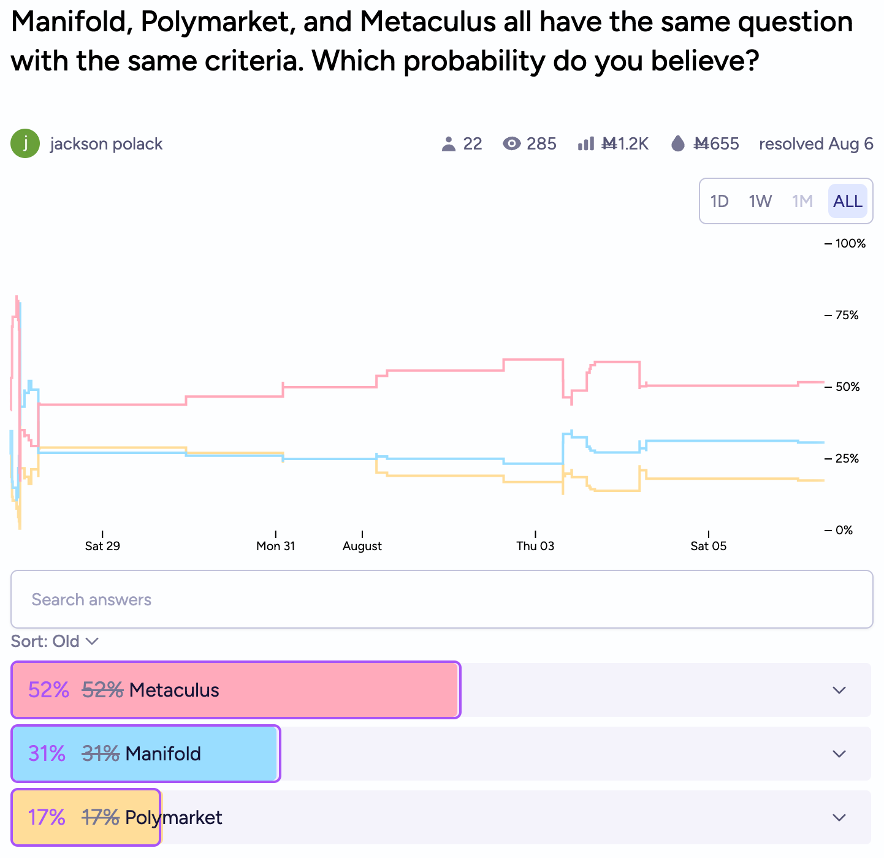
\includegraphics[scale=0.6]{img/MarketComparison.png}
    \caption{Comparison of the price of the same question in different predictive markets}
    \label{fig:market_comparison}
\end{figure}

This type of divergence is also common in cryptocurrencies predictive markets, because as the user bases and skill levels vary, so do market expectations and pricing. Furthermore, the efficiency of price adjustments is influenced by platform-specific variations in liquidity. Price disparities can also be caused by the dissemination and processing of information, transaction costs, and platform usability, as these factors can influence trader participation and market efficiency. These elements may contribute to the persistence of price disparities, particularly in more closed markets.

\subsection{Low Susceptibility to Manipulation}
\label{subsec:low_susceptibility_to_manipulation}

As defined by \cite{buckley2017effect}:
\begin{quote}
    \textit{A manipulation is an attempt by an individual or group of traders to affect the price of contracts being traded on a prediction market in a manner which contradicts their privately held information.}
\end{quote}
    
A prediction market can be manipulated when buyers of shares artificially inflate the demand for a false security regarding the fulfillment of a contract \parencite{choo2022manipulation}. If the results of such a predictive market are used to make policy decisions (exogenous manipulation), for example, the manipulating agents are willing to pay the cost that the deviation from the market prediction implies.
    
According to the literature on predictive markets, it is assumed that these are robust against manipulations. It is based on the argument that, if some agent tries to set a price that is not based on available information, another agent could take advantage of this deviation to make profits \parencite{buckley2017effect}.
    
According to \cite{HANSON2006449}, predictive markets can be subjected to experimentation, as a scenario with a defined set of information and incentives can be reproducible. When subjected to experimentation, studies confirm this hypothesis; however, one of the limitations in these experimental exercises is that participants may incur losses associated with manipulation exercises. This might be true in most predictive markets, but if the manipulating agents value the outcome of the manipulation more than the cost it implies, the hypothesis might not hold \parencite{deck2013affecting}.

In the study conducted by \citeauthor{HANSON2006449}, those agents who were incentivized to manipulate, set prices that were higher compared to those without incentives. However, in their experiment, this manipulation did not have a significant effect on equilibrium prices. Nevertheless, their results depends on the suspicion that the market is being manipulated, meaning that non-manipulating agents are aware of the possible attempt to manipulate and, therefore, correct their prices expectations.
    
On the other hand, \citeauthor{deck2013affecting} designs an experiment with two fundamental differences from that proposed by \Citeauthor{HANSON2006449}: \begin{enumerate*}[label=(\roman*)]
    \item the number of shares is not fixed, but any amount of shares can be bought or sold, and
    \item the manipulating agents have perfect information, and their profits do not depend on the number of shares they hold, but on the market outcome itself.
\end{enumerate*} 
The second point makes manipulators have the maximum incentive to intervene in the market. The conclusion of this study is that the presence of such manipulating agents makes the market unable to aggregate an accurate prediction. Additionally, in this study, it was determined that the manipulation strategy consists of increasing the volume of traded shares compared to the non-manipulated market, achieving this by emptying the Ask offers in the Order Book and, consequently, altering the equilibrium price.
\section{Conclusion}
\label{sec:conclusion}

\lipsum[2]


\section{References}
% the \nocite command leads to the whole bibliography
% being displayed (without any \cite commands necessary).
% remove this command in order to get the "normal" behavior.
\nocite{*}
\printbibliography[heading=none]
\end{document}
